\documentclass[a4paper,12pt]{article} % тип документа
\usepackage[margin=1in]{geometry} % Поля

%  Русский язык
\usepackage[warn]{mathtext}
\usepackage[T2A]{fontenc}			% кодировка
\usepackage[utf8]{inputenc}			% кодировка исходного текста
\usepackage[english,russian]{babel}	% локализация и переносы
% Математика
\usepackage{amsmath,amsfonts,amssymb,amsthm,mathtools} 
\usepackage{wasysym}
%%%
\usepackage{graphicx}
\usepackage{tabularx}


\usepackage{gensymb} % знак градуса
\usepackage{enumitem} % изменить список enumerate
\usepackage{placeins} % \FloatBarrier

\renewcommand{\thesection}{\Roman{section}} 
\renewcommand{\thesubsection}{\roman{subsection}}


\begin{document}
\newcolumntype{Y}{>{\centering\arraybackslash}X} %new tabularx

%титул
\hrule 	
\medskip
\begin{raggedright}
{\large \textbf{Отчёт по работе 3.1.3}}
\\
\medskip
{\Large Измерение магнитного поля Земли} 
\\
\medskip
{\large Карташов Констанин Б04-005}
\medskip
\hrule
\medskip
\end{raggedright}


\section{Анотация}

\paragraph{Цель работы:} 
\begin{enumerate}
\itemsep0em
\item Исследовать свойства постоянных неодимовых магнитов, 
\item Измерить с их помощью горизонтальную и вертикальную составляющие индукции
магнитного поля Земли и магнитное наклонение.
\end{enumerate}

\paragraph{Оборудование:}
\begin{itemize}
\renewcommand{\labelitemi}{$\triangleright$}
\itemsep0em
\item неодимовые магниты,
\item тонкая нить для изготовления крутильного маятника,
\item медная проволока,
\item электронные весы,
\item секундомер,
\item измеритель магнитной индукции,
\item штангенциркуль,
\item брусок, линейка и штатив из немагнитных материалов,
\item набор гирь и разновесов.
\end{itemize}


\medskip\hrule\medskip

\section{Теоретическая часть}

\paragraph{Магнитное поле Земли.} Земля имеет собственное магнитное поле, индукция которого влияет на микроскопические и макроскопические объекты, находящиеся в нём. Магнитное поле Земли локально можно представить в виде вектора магнитной индукции направленным к северному магнитному полюсу и имеющий некоторый угол наклона относительно горизонта.

\paragraph{Определение магнитного момента шарика.}
\paragraph{Метод А.} Сила притяжения двух одинаковых магнитных шариков:
\[ F = \frac{6P_m}{r^4} \; \text{(ед. СГС)}, \]
исходя из чего можно вычислить $P_m$, зная $F$ и $r$. 
\paragraph{Метод Б.} Сцепив несколько одинаковых магнитных шариков друг с другом, можно вычислить силу $F$, с которой верхний притягивает нижние к себе. Если принять $F_0$ за силу притяжения двух шариков:

\[ F_0 =frac{3P_m^2}{8R^4}, \; F = F_0 \left( 1 + \frac{1}{2^4} + \frac{1}{3^4} + \hdots \right) \approx 1.08 F_0. \]

\paragraph{Момент силы магнитной индукции.} Под действием магнитной индукции, тело с магнитным моментом испытывает момент силы $\vec{M} = \vec{P}_m \times \vec{B}$. Пользуясь этим свойством можно описать взаимодействие магнитного поля земли с магнитной стрелкой.


\medskip\hrule\medskip

\section{Экспериментальная часть}

\subsection{Определение магнитного момента, намагниченности и остаточной магнитной индукции вещества магнитных шариков.}

\paragraph{Метод А.} Измерим массу шарика цифровыми весами. Масса 12-ти шаров $m_{12} = 10.142 \pm 10^{-3}$ г, значит масса шарика $m = 0.8542 \pm 10^{-4}$ г. Измерим диаметр шарика штангенциркулем. Диаметр одного шарика $d = 0.6 \pm 0.01$ см. Используя дощечки и листочки бумаги, найдём максимальное расстояние на котором притягиваются шарики. Толщина прокладки $r_{\Pi} = 1.78 \pm 0.01$ см. Получаем максимальное расстояние $r_{\max} = d + d_{\Pi} = 2.38 \pm 0.02$ см. Расписав силы найдём момент магнитной индукции и индукцию шарика:
\[ F  = \frac{6 P_{\text{m}}}{r_{\max}^4} = mg \; \Rightarrow \; P_{m} = r_{\max}^2 \sqrt{\frac{mg}{6}}, \; 
B_{p} = \frac{2 P_{m}}{R^3} = \frac{2 r_{max}^2}{R^3}\sqrt{\frac{mg}{6}} \;\;\; \text{(ед. СГС)}.
\]

Подставим измеренные значения:

\[ P_m = 2.38^2 \sqrt{\frac{0.8542 \cdot 981.6}{6}} = 66.96 \; \frac{\text{эрг}}{\text{Гс}}, \;\;\; B_p = \frac{2 \cdot 66.96}{0.3^3} = 4960 \; \text{Гс}.
\]

Рассчитаем погрешности:

\[\sigma_P = P_m \sqrt{\left( 2 \frac{\sigma_r}{r_{\max}} \right)^2 + \left( \frac{1}{2} \frac{\sigma_m}{m} \right)^2} = 66.96 \sqrt{\left( 2 \frac{0.02}{2.38} \right)^2 + \left( \frac{1}{2} \frac{10^{-4}}{0.8542} \right)^2} = 1.1 \; \frac{\text{эрг}}{\text{Гс}},
\]

\[\sigma_B = B_p \sqrt{\left( \frac{\sigma_P}{P_m} \right)  + \left( 3 \frac{\sigma_R}{R} \right)^2} = 4960 \sqrt{\left( \frac{1.1}{70.0} \right)  + \left( 3 \frac{0.005}{0.3} \right)^2} = 260 \text{Гс}.
\]

Получили: $P_m = 70 \pm 1 \; \frac{\text{эрг}}{\text{Гс}}, \; B_p = 4960 \pm 260 \; \text{Гс}$.

\paragraph{Метод Б.} Сцепим несколько одинаковых магнитных шариков и подвесим к ним груз. Постепенно будем увеличивать массу грузов, до тех пор пока цепь из магнитных шариков не разорвётся. Измерим предельную массу отцепившейся от шарика части, $m = 329.7 \pm 0.1$ г. Сила сцепления двух магнитных шариков:

\[ F_0 = \frac{3 P_m^2}{8 R^4} \; \Rightarrow \; P_m = R^2 \sqrt{\frac{8F_0}{3}} \; \Rightarrow \; B_p = \frac{2}{R}\sqrt{\frac{8F_0}{3}} \;\;\; \text{(ед. СГС)}.
\]

Зная, что минимальный вес при котором цепочка оторвётся от верхнего шарика $F = 1.08F_0 = mg$, рассчитаем значения для $P_m$ и $B_p$:

\[ P_m = R^2 \sqrt{\frac{8F_0}{3}} = 2 R^2 \sqrt{\frac{mg}{1.62}} = 2 \cdot 0.3^2 \sqrt{\frac{329.7 \cdot 982}{1.62}} = 80.5 \frac{\text{эрг}}{\text{Гс}},
\]
\[ B_p = \frac{4}{0.3} \sqrt{\frac{329.7 \cdot 982}{1.62}} = 5960 \text{Гс}.
\]

Рассчитаем погрешность:

\[ \sigma_P = P_m \sqrt{\left( 2 \frac{\sigma_R}{R} \right)^2 + \left( \frac{1}{2} \frac{\sigma_m}{m} \right)^2} = 80.5 \sqrt{\left( 2 \frac{0.005}{0.3} \right)^2 + \left( \frac{0.1}{2 \cdot 329.7} \right)^2} = 2.7 \; \frac{\text{эрг}}{\text{Гс}},
\]
\[ \sigma_B = B_p \sqrt{\left( \frac{\sigma_R}{R} \right)^2 + \left( \frac{1}{2} \frac{\sigma_m}{m} \right)^2} = 5960 \sqrt{\left( 2 \frac{0.005}{0.3} \right)^2 + \left( \frac{0.1}{2 \cdot 329.7} \right)^2} = 100 \text{Гс}.
\]

Получили: $P_m = 81 \pm 3 \; \frac{\text{эрг}}{\text{Гс}}, B_p = 5960 \pm 100 \; \text{Гс}$.

\paragraph{} Измерим $B_p$ магнитометром. Получили $B_p = 270 \pm 10 \; \text{мТл} = 2700 \pm 100 \; \text{Гс}$.


\subsection{Измерение горизонтальной составляющей магнитного поля Земли.}

\paragraph{} Соберём магнитную стрелку из $n$ магнитных шариков, и подвесим её на $\Lambda$-образный подвес, чтобы в ней можно было возбудить крутильные колебания. Убедимся в том, что вкладом упругости в период колебаний можно пренебречь. Для этого вызовем крутильные колебания в кольце из 12 магнитных шариков. Сделав это видим, что крутильные колебания не возникают.

\paragraph{} Исследуем зависимость периода крутильных колебаний стрелки $T$ от количества шариков $n$:

\begin{table}[h]
\begin{center}
\begin{tabularx}{\textwidth}{|l||Y|Y|Y|Y|Y|}
\hline
$n$ & 3 & 4 & 5 & 6 & 7 \\ \hline
$T$ & 0.68 & 0.97 & 1.21 & 1.49 & 1.60 \\ \hline
\hline
$n$ & 8 & 9 & 10 & 11 & 12 \\ \hline
$T$ & 1.84 & 2.14 & 2.30 & 2.54 & 2.99 \\ \hline
\end{tabularx}
\end{center}
\end{table}

\paragraph{} Построим график зависимости $T(n)$ и проведём аппроксимирующую прямую пользуясь методом наименьших квадратов (полная формула представлена в первом томе лабораторного практикума). В частности, для расчёта коэффициента наклона прямой используются формулы:

\[
\kappa = \frac{\langle n \cdot T \rangle - \langle n \rangle \langle T \rangle}{\langle n^2 \rangle - \langle n \rangle ^ 2} = \frac{15.291 - 7.5 \cdot 1.776}{64.5 - 7.5 ^ 2} = 0.239 \; \text{с},
\]
\[
\sigma_\tau = \frac{1}{\sqrt{N}}\sqrt{\frac{\langle T^2 \rangle - \langle T \rangle ^ 2}{\langle n^2 \rangle - \langle n \rangle ^ 2} - k^2} = \frac{1}{\sqrt{10}}\sqrt{\frac{3.629 - 1.776 ^ 2}{64.5 - 7.5 ^ 2} - 0.239^2} = 0.007 \; \text{с}.
\]

\begin{figure}
\begin{center}
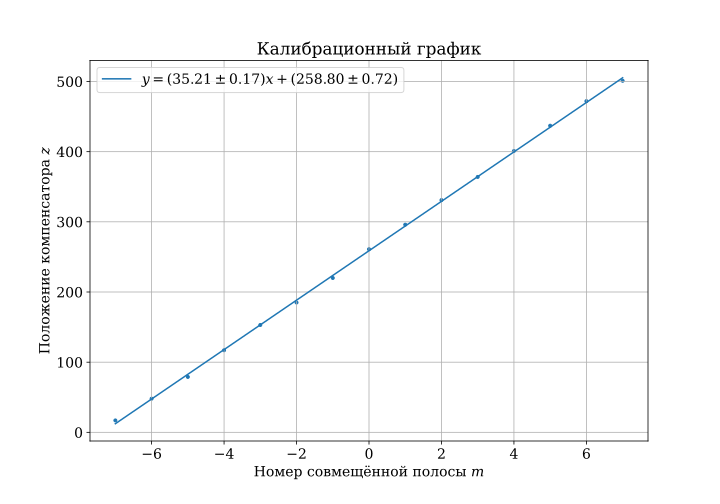
\includegraphics[width=6in]{plot1.png}
\caption{Первый график}
\label{plot1}
\end{center}
\end{figure}

По графику видим, что получившаяся прямая проходит через точку $(0,0)$, что соответствует ожиданию. Выражаем коэффициент наклона из формулы:
\[ \kappa = 2 \pi \sqrt{\frac{m R^2}{3 P_m B_\parallel}} = 2\pi \sqrt{\frac{m}{B_r R B_\parallel}} \Rightarrow B_\parallel = \frac{4 \pi^2 m}{\kappa^2 B_r R}.
\]

Подставим полученные и табличные значения в формулу:

\[ B_\parallel = \frac{4 \pi^2 \cdot 0.854}{0.239^2 \cdot 1.22 \cdot 10^{4} \cdot 0.3} = 1.61 \; \text{Гс}.
\]

Рассчитаем погрешность:

\[ \sigma_B = B_\parallel  \sqrt{\left( 2 \frac{\sigma_\kappa}{\kappa} \right)^2 + \left(  \frac{\sigma_R}{R} \right)^2 + \left(  \frac{\sigma_m}{m} \right)^2} = 1.61 \sqrt{\left(2 \frac{0.007}{0.239} \right)^2 + \left(\frac{0.01}{6} \right)^2 + \left( \frac{10^{-4}}{0.8542} \right)^2} = 0.09 \text{Гс}.
\]

Получаем $B_\parallel = 1.6 \pm 0.1$ Гс.

\subsection{Определение вертикальной составляющей магнитного поля Земли.}

\paragraph{} Соберём такую-же магнитную стрелку как в предыдущем разделе, но подвесим её в одной точке. Увидим, что магнитная стрелка находится под некоторым углом.

\paragraph{} Для различных значений $n$ уравновесим стрелку, и измерим приложенный момент сил $M_n$ при помощи весов дли измерения массы груза $m_n$ и известного диаметра шара для измерения плеча силы $r_n$ ($M_n = m_n g r_n$).

\begin{table}[h]
\begin{center}
\begin{tabularx}{0.5\linewidth}{|l|X|X|X|}
\hline
$n$ & $m_n$, г & $r_n$, см & $M_n$, дин$\cdot$см \\ \hline
4 & 0.205 & 0.6 & 121 \\ \hline
6 & 0.173 & 1.2 & 204 \\ \hline
8 & 0.173 & 1.2 & 204 \\ \hline
10 & 0.173 & 1.8 & 306 \\ \hline
12 & 0.176 & 3.0 & 518 \\ \hline
\end{tabularx}
\end{center}
\end{table}

\paragraph{} Построим график зависимости $M(n)$ и проведём аппроксимирую прямую пользуясь методом наименьших квадратов. Коэффициент наклона прямой $\alpha = 45 \pm 9$ дин$\cdot$см. Прямая пересекает ось $Oy$ в точке $(0,-88)$, что не соответствует формуле, из чего можно сделать вывод, что проведённые измерения неточные, что подтверждаете высокая погрешность  в коэффициенте наклона.

\begin{figure}
\begin{center}
\includegraphics[width=6in]{plot2.png}
\caption{Второй график}
\label{plot2}
\end{center}
\end{figure}

\paragraph{} Выразим коэффициент наклона из формулы:

\[ M_n = n P_m B_\perp = \frac{B_r R^3 B_\perp}{3}n \Rightarrow \alpha = \frac{B_r R^3 B_\perp}{3} \Rightarrow B_\perp = \frac{3 \alpha}{B_r R^3} = \frac{3 \cdot 45}{1.22 \cdot 10^{4} \cdot 0.3^3} = 0.4 \text{Гс},
\]

\[ \sigma_\alpha = B_\perp  \sqrt{\left( \frac{\sigma_\alpha}{\alpha} \right)^2 + \left(  3 \frac{\sigma_R}{R} \right)^2} = 0.4 \sqrt{\left( \frac{9}{45} \right)^2 + \left(  3 \frac{0.1}{6} \right)^2} = 0.08 \; \text{Гс}.
\]

Получаем $B_\perp = 0.4 \pm 0.08$ Гс.

\subsection{Магнитное наклонение и полная индукции магнитного поля Земли.}

\paragraph{} Полная индукция магнитного поля Земли равна $B = \sqrt{B_\parallel^2 + B_\perp^2} = \sqrt{1.61^2 + 0.4^2} = 1.66$ Гс. Погрешность $\sigma_B = \sqrt{\sigma_{B \parallel}^2 + \sigma_{B \perp}} = \sqrt{0.09^2 + 0.08^2} = 0.12$ Гс. Получаем значение $B = 1.66 \pm 0.12$ Гс. Вычислим магнитное наклонение $\beta$:

\[ \beta = \arctan{\frac{B_\perp}{B_\parallel}} = \arctan{\frac{0.4}{1.61}} = 0.24 = 14\degree
\]

\medskip\hrule\medskip

\section{Выводы}

\paragraph{} Мы качественно показали влияние магнитного поля Земли, на магнитные материалы, показали влияние вертикальной и горизонтальной компоненты магнитного поля. Показали на практике, что магнитный момент системы из магнитных шариков является суммой магнитных моментов всех шариков.

\paragraph{} Мы пронаблюдали неточности в измерении магнитного момента шарика. Все способы измерения магнитного момента дали различный результат. Это показывает, что при использовании этих методов необходимо уделять особое внимание внешним факторам.

\paragraph{} Факторы, которые могли повлиять на результат: неоднородность шариков, случайное смещение шариков руками, влияние нитки в подвесе на шарики.

\medskip\hrule\medskip

\end{document}
